\section{Типы шумов}

\textbf{Шум} -- разнообразные искажения на цифровых изображениях, обусловленные разного рода помехами.

В данной лабораторной работе мы рассмотрим наиболее распространенные модели шумов на примере воздействия их на изображения \ref{img:source}. 

\begin{figure}[ht!]
    \centering
    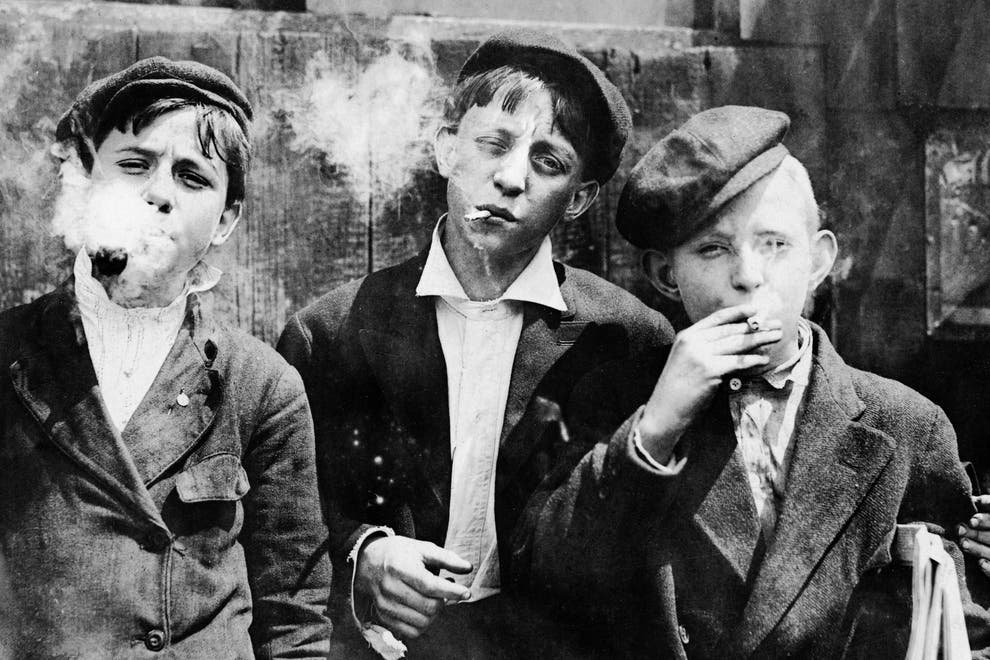
\includegraphics[width=\textwidth]{../lewis-hine-taschen-main-3.jpg}
    \caption{Исходное изображение}
    \label{img:source}  
\end{figure}
\FloatBarrier

\subsection{Импульсный шум}
Зашумленное изображение $I$ описывается следующей системой, причем значение интенсивности пикселя $I(x,y)$ будет изменено на значение $d \in [0,255]$:
\begin{equation}
    \begin{cases} d,\, \text{c вероятностью}\, p, \\
    s_{x,y},\, \text{c вероятностью}\, (1-p),
    \end{cases}
\end{equation}

где $s_{x,y}$ — интенсивность пикселя исходного изображения, если $d = 0$ — шум типа «перец», если
$d = 255$ — шум типа «соль».

\begin{figure}[ht!]
    \centering
    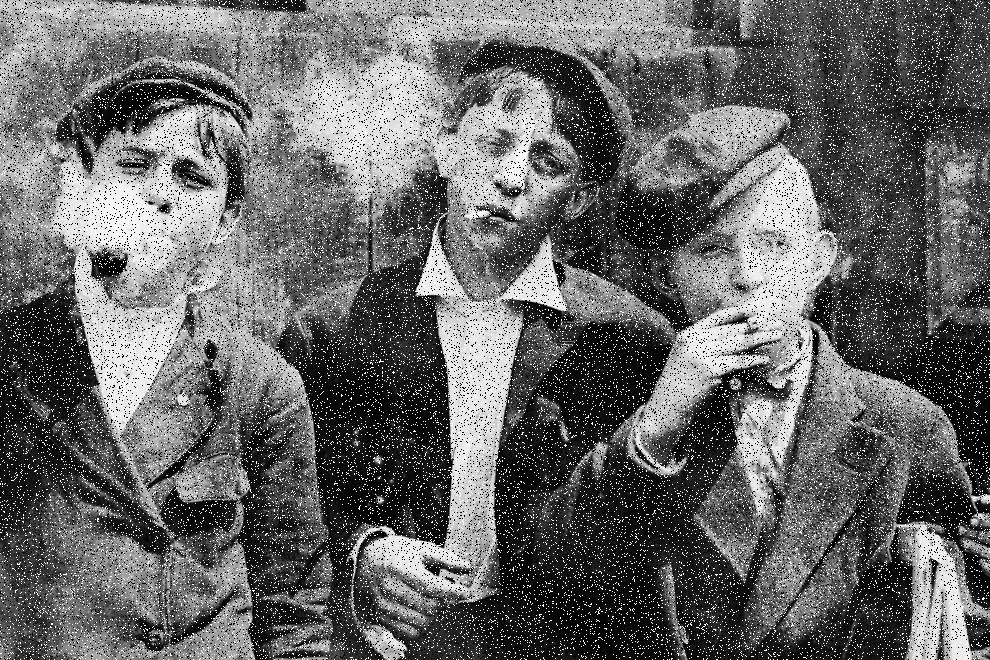
\includegraphics[width=\textwidth]{../Noisy_images/Impulse_noise.jpg}
    \caption{Результат воздействия импульсного шума на изображение \ref{img:source}}
    \label{img:impulse_noise}  
\end{figure}
\FloatBarrier

Итак, на изображении \ref{img:impulse_noise} отчетливо видны появившиеся белые («соль») и черные («перец») точки, что является характерным для импульсного шума, именно из-за этого он часто называется точечным шумом

\subsection{Аддитивный шум}
Аддитивный шум описывается следующим выражением:
\begin{equation}
    I_{new}(x,y) = I(x,y)  + \eta(x,y),
\end{equation}
где $ I_{new}$ — зашумленное изображение, $I$ — исходное изображение, $\eta$ — не зависящий от сигнала аддитивный шум с гауссовым или любым другим распределением функции плотности вероятности.

\begin{figure}[ht!]
    \centering
    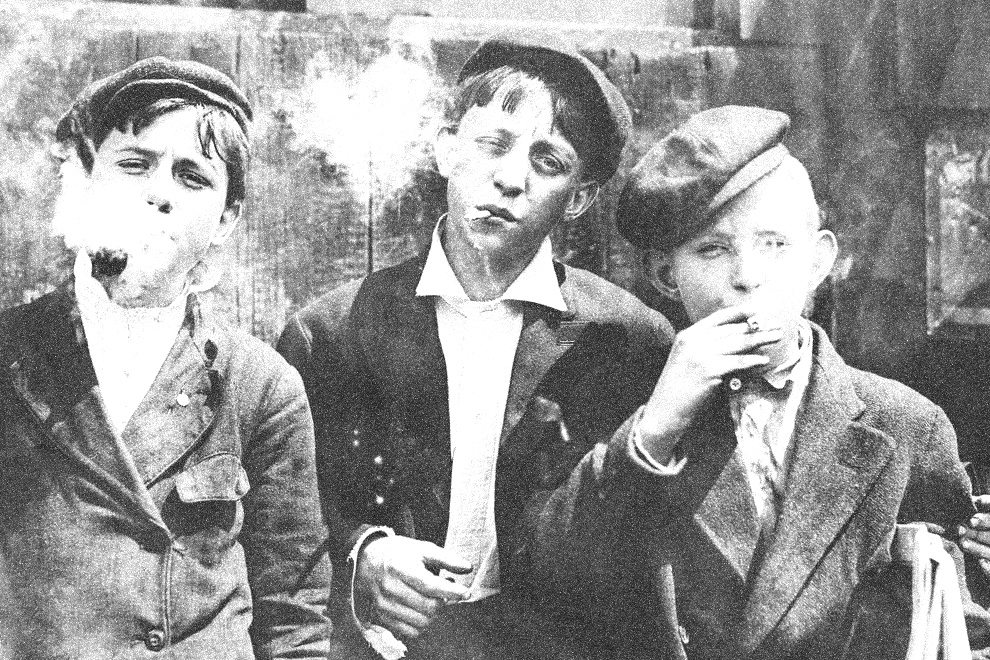
\includegraphics[width=\textwidth]{../Noisy_images/Additive_noise.jpg}
    \caption{Результат воздействия аддитивного шума на изображение \ref{img:source}}
    \label{img:additive_noise}
\end{figure}
\FloatBarrier

\subsection{Мультипликативный шум}
Мультипликативный шум описывается следующим выражением:
\begin{equation}
    I_{new}(x,y) = I(x,y) \cdot \eta(x,y),
\end{equation}

Частным случаем мультипликативного шума является спекл-шум, который мы и рассмотрим

\begin{figure}[ht!]
    \centering
    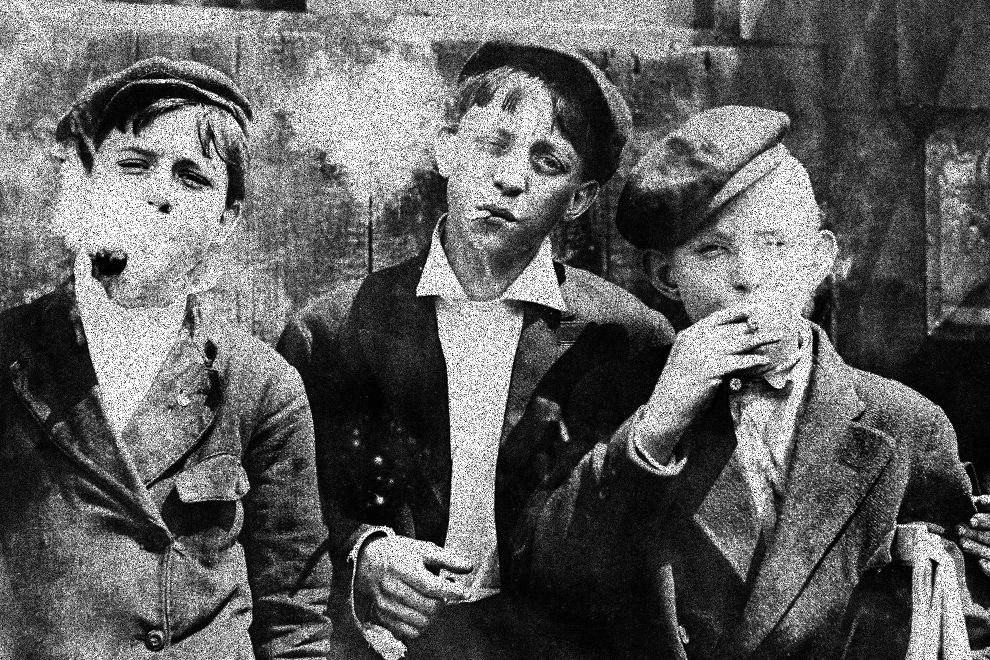
\includegraphics[width=\textwidth]{../Noisy_images/Speckle_noise.jpg}
    \caption{Результат воздействия спекл-шума на изображение \ref{img:source}}
    \label{img:speckle_noise}
\end{figure}
\FloatBarrier

\subsection{Гауссов (нормальный) шум}
Функция распределения плотности вероятности
$p(z)$ случайной величины $z$ описывается следующим выражением:
\begin{equation}
    p(z)= \frac{1}{\sigma\sqrt{2\pi}}\, e^{\frac{-(z-\mu)^2}{2\sigma^2}},
\end{equation}
где $z$ — интенсивность изображения (например, для полутонового изображения $z \in [0,255]$), $\eta$ — среднее (математическое ожидание) случайной величины $z$, $\sigma$ — среднеквадратичное отклонение, дисперсия $\sigma^2$ определяет мощность вносимого шума.


\begin{figure}[ht!]
    \centering
    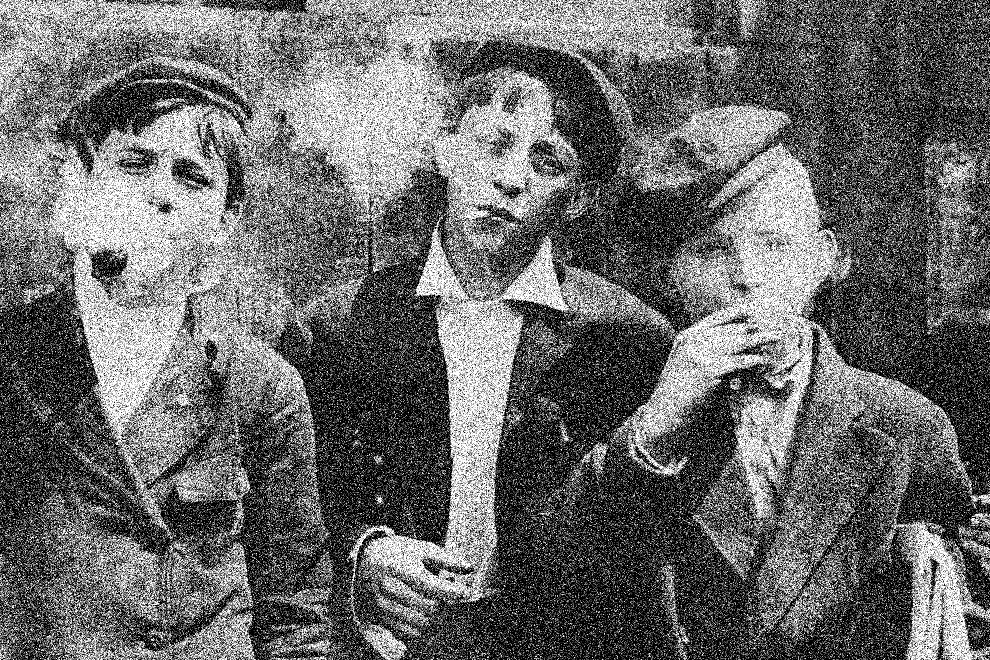
\includegraphics[width=\textwidth]{../Noisy_images/Gaussian_noise.jpg}
    \caption{Результат воздействия Гауссова шума на изображение \ref{img:source}}
    \label{img:gaussian_noise}
\end{figure}
\FloatBarrier


\subsection{Шум квантования}
Приближенно шум квантования можно описать распределением Пуассона. Такой шум не устраняется.

\begin{figure}[ht!]
    \centering
    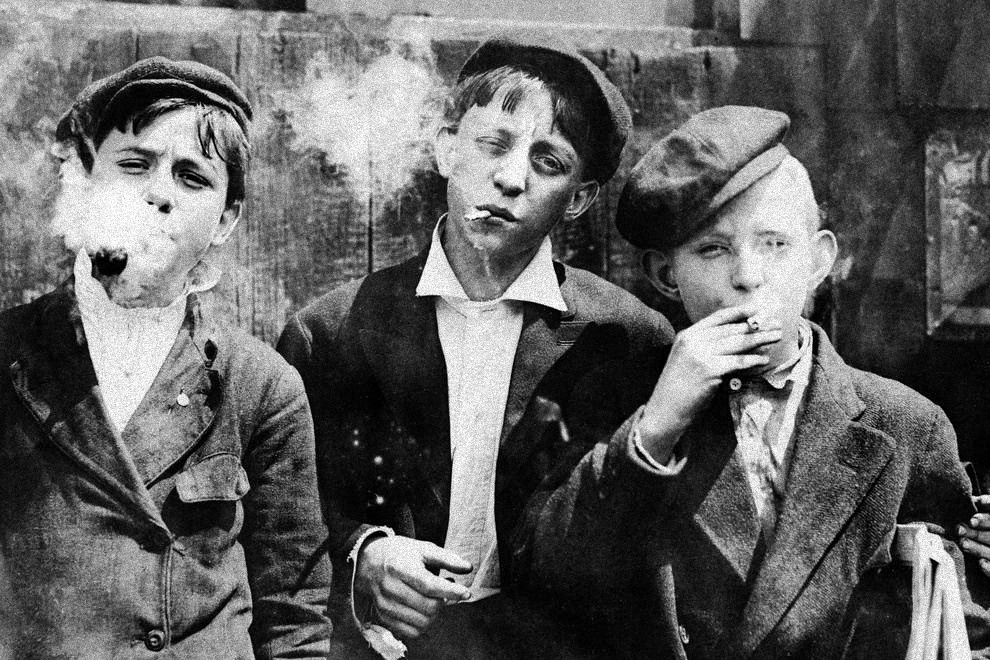
\includegraphics[width=\textwidth]{../Noisy_images/Poisson_Noise.jpg}
    \caption{Результат воздействия шума квантования на изображение \ref{img:source}}
    \label{img:poisson_noise}
\end{figure}
\FloatBarrier

\section{Фильтрация изображений}
\textit{Локальным} преобразованием называется такое преобразование, при котором для вычисления значения интенсивности каждого пикселя учитываются значения соседних пикселей в некоторой окрестности, называемой \textit{окном}, представляющей собой некоторую матрицу, которую также называют \textit{маской, фильтром, ядром фильтра}, а сами значения элементов
матрицы соответсвенно \textit{коэффициентами}. Как правило, маска имеет квадратную форму.

Фильтрация изображения $I$, имеющего размеры $M \times N$, с помощью маски размера $m \times n$ описывается формулой:
\begin{equation}
    I_{new}(x,y) = \sum_s \sum_t w(s,t) I(x+s,y+t),
\end{equation}
где $s$ и $t$ — координаты элементов маски относительно ее центра (в
центре $s = t = 0$). Такого рода преобразования называются \textit{линейными}.

\textit{Фильтрация в скользящем окне} — преобразование, при котором после вычисления нового значения интенсивности пикселя $I_{new}(x,y)$ окно $w$, в котором описана маска фильтра, сдвигается и
вычисляется интенсивность следующего пикселя.

\subsection{Низкочастотная фильтрация}
Низкочастотные пространственные фильтры ослабляют высокочастотные компоненты (области с сильным изменением интенсивностей) и оставляют низкочастотные компоненты изображения
без изменений. Отличительными особенностями
ядра низкочастотного фильтра являются: неотрицательные коэффициенты маски и то, что сумма всех коэффициентов равна единице.

\subsubsection{Контргармонический усредняющий фильтр}
Фильтр базируется на выражении:
\begin{equation}
    I_{new}(x,y) = \frac{\sum_{i=0}^m \sum_{j=0}^n I(i,j)^{Q+1}}{\sum_{i=0}^m \sum_{j=0}^n I(i,j)^Q}, \: \text{где $Q$ — порядок фильтра.}
\end{equation}


Рассмотрим применение фильтра при $Q > 0$, $Q < 0$ и
$Q = 0$.

\newpage

\subsubsection{Фильтр Гаусса}
При фильтрации изображений будем использовать двумерный фильтр Гаусса:
\begin{equation}
   G_\sigma = \frac{1}{2\pi\sigma^2} e^{-\frac{x^2+y^2}{2\sigma^2}} = \frac{1}{\sigma\sqrt{2\pi}} e^{\frac{-x^2}{2\sigma^2}} \cdot \frac{1}{\sigma\sqrt{2\pi}} e^{\frac{-y^2}{2\sigma^2}}
\end{equation}


\subsection{Нелинейная фильтрация}
\subsubsection{Медианная фильтрация}

\subsubsection{Взвешенная медианная фильтрация}
\subsubsection{Адаптивная медианная фильтрация}
\subsubsection{Ранговая фильтрация}
\subsubsection{Винеровская фильтрация}

\subsection{Высокочастотная фильтрация}
\subsubsection{Фильтр Робертса}
\newpage
\subsubsection{Фильтр Превитта}
\subsubsection{Фильтр Собела}
\subsubsection{Фильтр Лапласа}
\subsubsection{Алгоритм Кэнни}
\section{Выводы}

\section{Ответы на вопросы}

\newcounter{question}
\setcounter{question}{0}

\newcommand{\question}[1]{\item[Q\refstepcounter{question}\thequestion.] #1}
\newcommand{\answer}[1]{\item[A\thequestion.] #1}

\begin{itemize}

\question{В чем заключаются основные недостатки адаптивных методов фильтрации изображений?}
\answer{}

\question{При каких значениях параметра $Q$ контргармонический фильтр будет работать как арифметический, а при каких -- как гармонический?}
\answer{$Q$ — это порядок фильтра. Контргармонический фильтр является обобщением усредняющих фильтров. При $Q = 0$ фильтр превращается в арифметический, а при $Q = -1$ — в гармонический.}

\question{Какими операторами можно выделить границы на изображении?}
\answer{Можно выделить границы с использованием дифференциального оператора
Робертса.}

\question{Для чего на первом шаге выделения контуров, как правило, выполняется низкочастотная фильтрация?}
\answer{}

\end{itemize}
